\section{Informal Development}\label{sec:intuition}

We illustrate our \colosl  reasoning principles  by
sketching a proof of a variation of Dijkstra's token ring mutual
exclusion algorithm~\cite{dijkstra74}.  Consider the program
$\mathbb{INC}$ defined in \fig\ref{fig:concurrentInc}, ignoring the
assertions. It is written in pseudo-code resembling C with additional
constructs for concurrency: atomic sections $\atomic \_$ which
declare that code behaves atomically; and
parallel composition $\_ ||\_ $  which spawns threads then waits until
they complete. In our example, after
initialisation of the variables to $0$, three threads are spawned to
increment each variable in a lock-step fashion: $\mathbb{P}_{\li x}$
is the first allowed to run its increment operation; then
$\mathbb{P}_{\li y}$; and finally $\mathbb{P}_{\li z}$. This process
repeats until $\li{x} = \li{y} = \li{z} = 10$.  This example code is
interesting because the threads are intricately intertwined. With
thread $\mathbb{P}_{\li y}$, the programmer knows that the variables
\li{x} and
\li{y} are 
directly affected by the thread. He knows a simple behaviour of the thread that it will
increment variable  \li{y} as long as its value is less than that of \li{x}.
However, he also knows a much more complex behaviour  of the 
thread that, given the initial condition that all
the variables have value $0$, then the thread can only increase the
value of \li{y} by
$1$ if \li{x} is one more than \li{y},  and the environment can only
increase \li{x} by one if \li{x} and \li{z} (and in fact \li{y}) have
the same value. Finally, the programmer knows that the end result will
be that the value of all the variables will
be $10$. \colosl can simply specify   this complex
behaviour of the resource associated with thread $\mathbb{P}_{\li y}$.

\begin{figure*}
\centering
\begin{tabular}{@{}l@{\ }|@{\ }l@{\ }|@{\ }l@{\ }|@{\ }l@{}}
  {$\mathbb{P}_{\li x}$:}& 
  {$\mathbb{P}_{\li y}$:}& 
  {$\mathbb{P}_{\li z}$:}&
  $\mathbb{INC}$:\\[.5ex]
\begin{lstlisting}
//$\comment\{\shared{\cell{\tx z}{0} * \cell{\tx x}{0}}{I_{\tx x}} * [\token a_{\tx x}]\}$
while(x != 10)
//$\comment\left\{\shared{\begin{array}{@{}l<{\null}@{}l<{\null}@{}}\exsts{v}\cell{\tx z}{v} * \cell{\tx x}{v} \lor\\ \cell{\tx z}{v} * \cell{\tx x}{v+1}\end{array}}{I_{\tx x}}\!\!\!\!\!\! * [\token a_{\tx x}]\right\}$
{ $\langle$if (x == z) x++;$\rangle$ }
//$\comment\left\{\shared{\begin{array}{@{}l<{\null}@{}l<{\null}@{}}\cell{\tx z}{10} * \cell{\tx x}{10} \lor\\ \cell{\tx z}{9} * \cell{\tx x}{10}\end{array}}{I_{\tx x}}\!\!\!\!\!\! * [\token a_{\tx x}]\right\}$
\end{lstlisting}
&
\begin{lstlisting}
//$\comment\left\{\shared{\begin{array}{@{}l<{\null}@{}l<{\null}@{}}\cell{\tx x}{0} * \cell{\tx y}{0} \lor\\ \cell{\tx x}{1} * \cell{\tx y}{0}\end{array}}{I_{\tx y}}\!\!\!\!\!\! * [\token a_{\tx y}]\right\}$
while(y != 10)
//$\comment\left\{\shared{\begin{array}{@{}l<{\null}@{}l<{\null}@{}}\exsts{v}\cell{\tx x}{v} * \cell{\tx y}{v} \lor\\ \cell{\tx x}{v+1} * \cell{\tx y}{v}\end{array}}{I_{\tx y}}\!\!\!\!\!\! * [\token a_{\tx y}]\right\}$
{ $\langle$if (y < x) y++;$\rangle$ }
//$\comment\left\{\shared{\begin{array}{@{}l<{\null}@{}l<{\null}@{}}\cell{\tx x}{10} * \cell{\tx y}{10} \lor\\ \cell{\tx x}{11} * \cell{\tx y}{10}\end{array}}{I_{\tx y}}\!\!\!\!\!\! * [\token a_{\tx y}]\right\}$
\end{lstlisting}
&
\begin{lstlisting}
//$\comment\left\{\shared{\begin{array}{@{}l<{\null}@{}l<{\null}@{}}\cell{\tx y}{0} * \cell{\tx z}{0} \lor\\ \cell{\tx y}{1} * \cell{\tx z}{0}\end{array}}{I_{\tx z}}\!\!\!\!\!\! * [\token a_{\tx z}]\right\}$
while(y != 10)
//$\comment\left\{\shared{\begin{array}{@{}l<{\null}@{}l<{\null}@{}}\exsts{v}\cell{\tx y}{v} * \cell{\tx z}{v} \lor\\ \cell{\tx y}{v+1} * \cell{\tx z}{v}\end{array}}{I_{\tx z}}\!\!\!\!\!\! * [\token a_{\tx z}]\right\}$
{ $\langle$if (z < y) z++;$\rangle$ }
//$\comment\left\{\shared{\begin{array}{@{}l<{\null}@{}l<{\null}@{}}\cell{\tx y}{10} * \cell{\tx z}{10} \lor\\ \cell{\tx y}{11} * \cell{\tx z}{10}\end{array}}{I_{\tx z}}\!\!\!\!\!\! * [\token a_{\tx z}]\right\}$
\end{lstlisting}
&
{\hspace*{.8em}\begin{lstlisting}[numbers=left,numbersep=3pt]
//$\comment\{\tx x|-> - * \tx{y}|-> - * \tx{z}|-> - \}$
x = 0; y = 0; z = 0;
//$\comment\{\tx x|-> 0 * \tx{y}|-> 0 * \tx{z}|-> 0 \}$
//$\comment\left\{\begin{array}{@{}l<{\null}@{}l<{\null}@{}}\shared{\tx x|-> 0 * \tx{y}|-> 0 * \tx{z}|-> 0} I\\ \null*[\token a_{\tx x}] * [\token a_{\tx y}] * [\token a_{\tx z}]\end{array}\right\}$
($\mathbb{P}_{\tx x}$ || $\mathbb{P}_{\tx y}$ || $\mathbb{P}_{\tx z}$)
//$\comment\left\{\begin{array}{@{}l<{\null}@{}l<{\null}@{}}\shared{\tx x|-> \!\!10 * \tx{y}|-> \!\!10 * \tx{z}|-> \!\!10} I\\ \null*[\token a_{\tx x}] * [\token a_{\tx y}] * [\token a_{\tx z}]\end{array}\right\}$
\end{lstlisting}}
%\lstset{numbers=none}
\end{tabular}

\begin{minipage}{.2\textwidth}
\begin{align*}
  I_{\li x} &\eqdef \left\{
  \begin{array}{@{}l@{}}
    \token a_{\li x}:\, \exsts{v} \cell{\li{z}}{v} * \cell{\li{x}}{v}  \swap  \cell{\li{z}}{v} * \cell{\li{x}}{v+1}\\
    \token a_{\li z}:\, \exsts{v} \cell{\li{x}}{v+1} * \cell{\li{y}}{v+1} * \cell{\li{z}}{v}\swap \cell{\li{x}}{v+1} * \cell{\li{y}}{v+1} * \cell{\li{z}}{v+1}
  \end{array}
  \right.\\
  I_{\li y} &\eqdef \left\{
  \begin{array}{@{}l@{}}
    \token a_{\li x}:\, \exsts{v} \cell{\li{x}}{v} * \cell{\li{y}}{v} * \cell{\li{z}}{v}  \swap  \cell{\li{x}}{v+1} * \cell{\li{y}}{v} * \cell{\li{z}}{v}\\
    \token a_{\li y}:\, \exsts{v} \cell{\li{x}}{v+1} *  \cell{\li{y}}{v}\swap \cell{\li{x}}{v+1} * \cell{\li{y}}{v+1}
  \end{array}
  \right.\\
  I_{\li z} &\eqdef \left\{
  \begin{array}{@{}l@{}}
    \token a_{\li y}:\, \exsts{v} \cell{\li{x}}{v+1} * \cell{\li{y}}{v} * \cell{\li{z}}{v}  \swap \cell{\li{x}}{v+1} * \cell{\li{y}}{v+1} * \cell{\li{z}}{v}\\
    \token a_{\li z}:\, \exsts{v} \cell{\li{y}}{v+1} *  \cell{\li{z}}{v}\swap \cell{\li{y}}{v+1} * \cell{\li{z}}{v+1}
  \end{array}
  \right.
\end{align*}
\end{minipage}\quad\ 
\begin{minipage}{.2\textwidth}
\begin{align*}
  I &\eqdef \left\{
  \begin{array}{@{}l@{\,}l@{}l@{}}
    \token a_{\li x}: & \exsts{v} & \cell{\li{z}}{v} * \cell{\li{x}}{v} \swap\\
    &&\quad \cell{\li{z}}{v} * \cell{\li{x}}{v+1}\\
    \token a_{\li y}: & \exsts{v} & \cell{\li{x}}{v+1} * \cell{\li{y}}{v} \swap \\
    &&\quad \cell{\li{x}}{v+1} * \cell{\li{y}}{v+1}\\
    \token a_{\li z}: & \exsts{v} & \cell{\li{y}}{v+1} * \cell{\li{z}}{v} \swap \\
    &&\quad \cell{\li{y}}{v+1} * \cell{\li{z}}{v+1}
  \end{array}\right.
\end{align*}
\end{minipage}

\vspace{5pt}\hrule\vspace{5pt}
\caption{The concurrent increment program together with a \colosl proof
  sketch. Lines starting with \lstinline{//} contain formulas that describe
  the local state and the subjective shared state at the relevant program point.}
\label{fig:concurrentInc}
\end{figure*}





Now consider the \colosl assertions accompanying  $\mathbb{INC}$.
After
initialisation, line~3 of $\mathbb{INC}$  provides a standard
assertion from separation logic~\cite{seplog} with variables as
resource~\cite{variablesAsResource}. The assertion  declares  that the variable cells
addressed by 
\li{x},
\li{y} and \li{z}  have the same value  $0$. This variable resource in the thread-local state is
fully owned by  the thread. Using the \extendRule\ principle, the thread is able to give up  this local
resource and transfer it  to the global shared state. For example,
line~4 demonstrates the
creation of a subjective view $\shared{\li{x}|-> 0 * \li{y}|-> 0 * \li{z}|->
  0}I$, where {part} of the underlying
global shared state now contains the three variable  cells and the 
interference relation $I$ declares  how  this  part of the  shared state can change. For example,  the action 
\[
 \token a_{\li y}:  \exsts{v} \cell{\li{x}}{v+1} * \cell{\li{y}}{v} \swap 
 \cell{\li{x}}{v+1} * \cell{\li{y}}{v+1}
\]
can increment  the variable cell  \li{y} under the condition that the
value of the  cell
given by \li{x} is one more than that of \li{y}. 
This update is only possible when the
local state of a thread has the { capability} $[\token a_{\li y}]$. For  this
particular 
example, the assertion in line~4 simply has all the capabilities $[\token
a_{\li x}] * [\token a_{\li y}] * [\token a_{\li z}]$ of the $I$-actions   in the local state; in general,
capabilities can be buried inside boxes, only to emerge as a
consequence of an action
(see \S\ref{sec:examples}). 



Using the 
\copyRule\ principle for subjective views and the disjoint concurrency
rule, we obtain a  precondition for thread $\mathbb{P}_{\li y}$:
\[
\shared{\li{x}|-> 0 * \li{y}|->0 * \li{z}|-> 0}{I} *[\token a_{\li y}]
\]
However, this precondition is more complicated than we
need. Intuitively, the specification of each thread should only use
the variable resource relevant to that thread, and need only consider actions
that affect that resource.  In this example, the extraneous piece of
state is the variable cell  \li{z}. This additional resource  might seem an acceptable
price to pay, but straightforward generalisations to $n$ participants
yields extra state of $n-2$ variable cells with  their associated
interferences which are of no interest to the particular thread.
Fundamentally, for large systems, the burden of carrying the whole
shared state around to analyse all threads,  can lead to intractable proofs.

As a first try at simplifying the precondition, consider the following implication using the \forgetRule\
and \shiftRule\ principles given in the introduction:
%
\[
\begin{array}{c l}
 & \shared{\li{x}|-> 0 * \li{y}|->0 * \li{z}|-> 0}{I} *[\token a_{\li y}]\\
\stackrel{(\forgetRule)}{=>}  &\shared{\li{x}|-> 0 * \li{y}|->0}{I} *[\token a_{\li y} ]\\
 \stackrel{(\shiftRule)}{\semimplies}  &\shared{\li{x}|-> 0 * \li{y}|->0 }{I\backslash\token a_{\li z}} *[\token a_{\li y}]\\
\stackrel{(\stabilise)}{=>}  &\shared{\exists v, v'.  (\li{x}|-> v * \li{y}|->v' ) \wedge v\geq v'}{I\backslash \token a_{\li z}} *[\token a_{\li y}]\\
\end{array}
\]
The thread $\mathbb{P}_{\li y}$ does not modify \li{z} and we can thus
forget the variable assertion $\li{z} \mapsto 0$. The variable cell addressed by \li{z} is no longer visible to $\mathbb{P}_{\li y}$ and the
action $\token a_{\li z}$ does not affect the resources described by the
assertion of the subjective view neither in its current state nor at any point during its lifetime. That is, the current subjective view is unaffected by $\token a_{\li z}$, and after undergoing any number of actions
from $I$, the resulting subjective view remains unaffected by $\token
a_{\li z}$. Using the \shiftRule\  principle, we
can therefore forget the $\token{a}_{\li z}$ action. 
Finally, as is normal when reasoning about concurrency, we weaken so
that, whatever the environment can do to the state, the assertion
inside the box still holds (the assertion is \emph{stable}). However, we have   lost information about
\li{z}. Intuitively, we know that the value of \li{y} depends on the value
of \li{z}, but there is nothing now to constrain \li{z}. Hence, we can only
stabilise in a general way as given, losing information about how the
values of \li{x} and \li{y} are connected together through \li{z}.

It is however possible to give a  stronger specification, as follows: 
\[
\begin{array}{c l}
 & \shared{\li{x}|-> 0 * \li{y}|->0 * \li{z}|-> 0}{I} *[\token a_{\li y}]\\
 
\stackrel{(\shiftRule)}{\semimplies} &  \shared{\li{x}|-> 0 * \li{y}|->0 * \li{z}|-> 0}{I'_{\li y}} *[\token a_{\li y} ]\\

 \stackrel{(\forgetRule)}{=>} & \shared{\li{x}|-> 0 * \li{y}|->0 }{I'_{\li y}} *[\token a_{\li y}]\\
 
\stackrel{(\shiftRule)}{\semimplies} &  \shared{\li{x}|-> 0 * \li{y}|->0 }{I_{\li y}} *[\token a_{\li y}] \\
\stackrel{(\stabilise)}{=>} &
    \shared{\begin{array}{@{}l<{\null}@{}l<{\null}@{}}\cell{\li{x}}{0} *
        \cell{\li{y}}{0} \lor\\ \cell{\li{x}}{1} *
        \cell{\li{y}}{0}\end{array}}{I_{\li y}}\!\!\!\!\!\! * [\token a_{\li y}]
\end{array}
\]
This implication involves subtle interaction between the assertion and
the interference relation of the subjective view. 
Consider the action 
$\token a_{\li x}$ 
of $I$ and the initial state with value $0$ in all the cells. This
action can be replaced by:
\[
\token a_{\li x} : \exsts{v} \; 
\cell{\li{x}}{v} * \cell{\li{y}}{v} * \cell{\li{z}}{v}
\swap
\cell{\li{x}}{v+1} * \cell{\li{y}}{v} * \cell{\li{z}}{v}
\]
This is possible  because, as the programmer knows, whenever the cells
of \li{x} and
\li{z} have the same value then the \li{y} cell also has the same value which, under these
conditions, is not changed by the actions in $I$. This amended action  gives full information about how the resource of
the subjective view changes as \li{x} is being updated.
Let  $I_{\li y}' $ be  $I_{\li y}$ with $\token a_{\li x}$ rewritten as above.
As we justify in \S~\ref{sec:logic}, we can 
use  the \shiftRule\ principle with the following judgement judgement 
$
I\weakenIb{\cell{\li{x}}{0} * \cell{\li{y}}{0} * \cell{\li{z}}{0}} I_{\li y}'
$
to replace $I_{\li y}$ by $I'_{\li y}$. 

Using \forgetRule,  it is now safe to lose the \li{z} cell to
obtain the subjective view  $\shared{\li{x}|-> 0 * \li{y}|->0 }{I'_{\li y}}$,  as 
the new $\token a_{\li x}$ action in $I'_{\li y}$ retains enough information about how
\li{x}, \li{y} and \li{z} are related.
Since action $\token a_{\li z}$ only affects the \li{z} cell, which has been
forgotten, leaving  the cells \li{x} and \li{y} unaltered, we can again use the
\shiftRule\ principle to change  the interface
relation to $I_{\li y} = I'_{\li y} \backslash \token a_{\li z}$. The interface relation
is now as simple as it can get, whilst retaining enough information
about the 
connection between the \li{x}, \li{y} and \li{z}. We weaken
the 
assertion $\li{x}|-> 0 * \li{y}|->0$ to make it stable with respect to $I_{\li y}$ and obtain our final
precondition of thread $\mathbb{P}_{\li y}$, which retains much more
information about the values of the \li{x} and \li{y} cells. 







There is one more subtlety to mention about this precondition.  The
thread has the capability $[\token a_{\li y}]$ to perform action $\token
a_{\li y}$ which only requires the resource described by the
assertion. However, the action $\token a_{\li x}$ depends on the
resource given by \li{z}, which is no longer a part of the subjective view
of the thread. Since another thread in the environment may own the $[\token{a_{\li x}}]$ capability, it may perform the $\token{a_{\li x}}$ action whenever its subjective view is {\em compatible} with the pre-condition of the action.
When that is the case, the piece of the
state corresponding to the overlap between the state and the
precondition of the action is removed, and the entire postcondition of
the action is added in its place. Diagrammatically, a subjective state
(represented by the circle) is affected as follows by an action $P\swap Q$:
\[
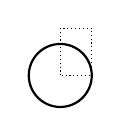
\begin{tikzpicture}[baseline]
\draw[thick] (0,0) circle (.4cm);
\draw[densely dotted] (0,0) rectangle (.4cm,.6cm);
\end{tikzpicture}
\quad\swap\quad
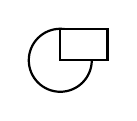
\begin{tikzpicture}[baseline]
\draw[thick] (0,0) circle (.4cm);
\draw[thick,fill=white] (0,0) rectangle (.6cm,.4cm);
\end{tikzpicture}
\qquad
\left(\text{where }
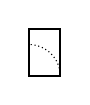
\begin{tikzpicture}[baseline,yshift=-.25cm]
\draw[thick] (0,0) rectangle (.4cm,.6cm);
\draw[densely dotted] (.4cm,0) arc (0:90:.4cm);
\end{tikzpicture}|= P
\text{ and }

\begin{tikzpicture}[baseline]
\draw[thick,yshift=-.1cm] (0,0) rectangle (.6cm,.4cm);
\end{tikzpicture}|= Q\right)
\]
This is a direct consequence of the fact that the subjective view
describes the thread's partial knowledge about the shared state, while
the environment may have both the knowledge that the thread
has, as well as some additional knowledge. In this case, while the thread
does not have the capability to do action $\token a_{\li x}$, the
environment might.




The proof of the specification of the thread $\mathbb{P}_{\li y}$ is 
now relatively straightforward. By inspection, the invariant of the while loop is stable
with respect to $I_{\li y}$. The atomic section allows safe
manipulation of the contents of the subjective region.
 The final postcondition of $\mathbb{P}_{\li y}$ follows from the
invariant and the boolean expression of the while. We join up the
postconditions of the threads using the \mergeRule\ principle. Since $|/$
distributes over $**$, the subjective view simplifies to $
\shared{\li{x}|->10 * \li{y}|->10 * \li{z}|->10}{I_{\li x}\cup I_{\li y}\cup I_{\li z}} $.
Finally, we have 
\[
I_{\li x}\cup I_{\li y}\cup I_{\li z}\weakenIb{\li{x}|->10 * \li{y}|->10 * \li{z}|->10} I
\]
so, by the \shiftRule\ principle, we get the postcondition of $\mathbb{INC}$. 


%\paragraph{Comparison with other formalisms}
This concludes our \colosl proof of $\mathbb{INC}$. Using subjective
views and manipulating the interference assertions in key places
enables the specification and verification of each thread to be
confined to just the resources they need, a feat that is not possible
using previous work.

\paragraph{\colosl reasoning}
We complete our semi-formal overview with features of \colosl not
showcased by the proof above. First, we note that an action $P\swap Q$
may in general performs three actions: (1)
%% \begin{enumerate}
%% \item
  \emph{modify} resources: $P$ and $Q$ contain the same amount of
  resource with different values, \textit{e.g.}
  $\token{a}_{\tx{x}}$ in $I$;
%%\item
  (2)
  \emph{remove} resources from the shared state and move them into
  the local state of the thread performing the action, for instance
  when $P = Q * R$ for some resource to be removed $R$;
%%\item
  (3)
  conversely, \emph{add} resources from the local state of the thread
  into the shared state; the added resources only appears in $Q$,
  \textit{e.g.} $Q = P * R$.
%%\end{enumerate}   
We demonstrate the latter two behaviours through our examples in
\S\ref{subsec:CSTExample}. These three behaviours are not mutually
exclusive and an action may exhibit any combination of them.  Unlike
CAP~\cite{cap-ecoop10} and as in iCAP~\cite{icap}, we do not provide
an explicit \emph{unsharing} mechanism to claim shared
resources and render them thread-local. Instead, this behaviour can
be simply encoded as an additional action with the second behaviour
described above.

We also note that, as in the CAP family~\cite{cap,icap,tada}, \colosl
cannot ensure that proved programs do not leak memory. Indeed, one may
at any point of a proof stash leaked resources into a new subjective
view, then weaken the resulting assertion to remove that view from the
current state, rendering the leak invisible as far as the proof system
is concerned.

%% This finishes the justification of all uses of \eqref{eq:shift} in the
%% derivations of \S\ref{subsec:threads}, and thus the derivations
%% themselves.  In this section, we have informally justified
%% manipulations of the interference relation by semantic
%% arguments. However, \S\ref{sec:shiftax} will show how the reasoning
%% involved can be reduced to simple logical implications between
%% separation logic formulas that do not mention the shared state.



%% In the case of the less local predicate $G$, whenever the
%% pre-condition of the action associated with $\token a_{\li z}$ is satisfied
%% (third disjunct), it is also the case that $\cell{\li{x}}{v+1}$. In other
%% words, in all the cases where the shared state satisfies
%% $\cell{\li{y}}{v+1} * \cell{\li{z}}{v}$, it also satisfies $\cell{\li{x}}{v+1} *
%% \cell{\li{y}}{v+1} * \cell{\li{z}}{v}$. However, this information is not
%% reflected in $I$ and as a result when weakening $G$, we need to
%% stabilise the resultant assertion which proves to be very weak. To
%% remedy this, in \colosl we introduce the notion of action
%% \emph{shifting} (rewriting) with respect to the \emph{invariant} of
%% the shared state. Given $\shared{P}{I'}$, we write $\fence{} \fences
%% (P, I')$ - read ``$\fence{}$ fences $P$ with respect to $I'$'' - to
%% indicate that i) $\fence{}$ contains all states associated with $P$
%% and ii) it is closed under $I'$; that is, given any action in $I'$
%% whose pre-condition is satisfied by a state in $\fence{}$, the state
%% resulting from the action is also in $\fence{}$. For instance, given
%% the $G$ predicate of \fig\ref{fig:concurrentIncCoLoSLSpec}, we have
%% $\fence{G} \fences (P_G, I)$ where $P_G$ denotes the assertion inside
%% the box and $\fence{G}$ is as specified below.
%% \[
%% 	\begin{array}{l l}
%% 		\fence{G} = \hspace*{-5pt}& \left\{\cell{\li{x}}{v} * \cell{\li{y}}{v} * \cell{\li{z}}{v} ||| v \in \{0, \cdots 10\} \right\} \\
%% 		& \cup \left\{\cell{\li{x}}{v+1} * \cell{\li{y}}{v} * \cell{\li{z}}{v} ||| v \in \{0, \cdots 9 \} \right\} \\
%% 		& \cup \left\{\cell{\li{x}}{v+1} * \cell{\li{y}}{v+1} * \cell{\li{z}}{v} ||| v \in \{0, \cdots 9\} \right\}\\
%% 	\end{array}
%% \]
%% %as well as the action associated with its update
%% Given the above invariant, we can now \emph{shift} the action associated with $\token a_{\li z}$ in $I$ and arrive at $I'$ where
%% \[
%% 	I' \eqdef \left\{
%% 		\begin{array}{@{}l@{}}
%% 			\token a_{\li x}:\, \exsts{v} \cell{\li{x}}{v} * \cell{\li{z}}{v}  \swap  \cell{\li{x}}{v+1} * \cell{\li{z}}{v}\\
%% 			\token a_{\li y}:\, \exsts{v} \cell{\li{x}}{v+1} * \cell{\li{y}}{v}  \swap  \cell{\li{x}}{v+1} * \cell{\li{y}}{v+1}\\
%% 			\token a_{\li z}:\, \exsts{v} \cell{\li{x}}{v+1} *
%%                         \cell{\li{y}}{v+1} * \cell{\li{z}}{v} \swap\null\\
%% 			\hspace*{2cm} \cell{\li{x}}{v+1} * \cell{\li{y}}{v+1} * \cell{\li{z}}{v+1}\\
%% 		\end{array}			
%% 	\right.
%% \]
%% Note that in doing so we have neither restricted nor relaxed the action of $\token a_{\li z}$ in that it can be carried out in exactly the same states given the invariant $\fence{G}$. This is formalised by the \shiftRule\ rule where $I \weakenI{\fence{}} I'$ denotes the shifting of $I$ with respect to $\fence{}$ and we defer its formalisation to \S\ref{sec:logic}.
%% \[
%% 	\text{if}\hspace*{0.25cm} \fence{} \fences (P, I) 
%% 	\hspace*{0.25cm}\text{and}\hspace*{0.25cm} I \weakenI{\fence{}} I'
%% 	\hspace*{0.25cm}\text{then}\hspace*{0.25cm}
%% 	\shared{P}{I} ===> \shared{P}{I'} \hspace*{0.5cm} \shiftRule
%% \]
%% Given predicate $G$ of \fig\ref{fig:concurrentIncCoLoSLSpec}, we can first shift $I$ into $I'$ (specified above) using the \textsc{Shift} rule and then apply the \forgetRule\ rule to forget variable \li{y} and obtain $\shared{a_{\li x}}{I'}$.
%% %%
%% %\[
%% %	X' \eqdef \shared{\exsts{v} \cell{\li{x}}{v} * \cell{\li{z}}{v} \lor \cell{\li{x}}{v+1} * \cell{\li{z}}{v}}{I'} 
%% %\]
%% %%
%% We have almost arrived at a local specification for $\mathbb{P}_{\li x}$. However, the action of $\token a_{\li y}$ is still visible in $I'$ even though it does not affect the values of \li{x} or \li{z}. Through interference shifting, we can not only rewrite actions with respect to the invariant, we can also \emph{forget} actions that affect \emph{none} of the states contained in the invariant. For instance, let $\fence{\li{x}} = \left\{\cell{\li{x}}{v} * \cell{\li{z}}{v} ||| v \in \{0, \cdots 10\} \right\} \cup \left\{\cell{\li{x}}{v+1} * \cell{\li{z}}{v} ||| v \in \{0, \cdots 9 \} \right\}$, then we have $\fence{X} \fences (X, I')$. In the case of the action of $\token a_{\li y}$, given any state $p$ in the action pre-condition (e.g. $p = \cell{\li{x}}{1} * \cell{\li{y}}{0}$), for an arbitrary state $s \in \fence{X}$ (e.g. $s = \cell{\li{x}}{1} * \cell{\li{z}}{0}$), \emph{all overlaps} of $p$ and $s$ ($p \meetL s = \{\cell{\li{x}}{1}\}$) are preserved by the action. We give the formal definition of overlap operator $\meetL$ in \S\ref{sec:logic}. 

%% Given $I'$ and $\fence{X}$ we can again apply the \textsc{Shift} rule in order to forget about the action of $\token a_{\li y}$ and obtain $I_{\li x}$ as specified in \fig\ref{fig:concurrentIncSubjectiveSpec}. We can take analogous steps in order to obtain subjective views $S_{\li y}$ and $S_{\li z}$ for threads $\tau_{\li y}$ and $\tau_{\li z}$. We then pass the $\token a_{\li x}$, $\token a_{\li y}$ and $\token a_{\li z}$ capabilities to $\tau_{\li x}$, $\tau_{\li y}$ and $\tau_{\li z}$ and verify $\mathbb{INC}$ as follows:
%% \[
%% \hspace*{-0.2cm}
%% \begin{array}{c}
%% 	\color{blue}{\left\{\token a_{\li x} * \token a_{\li y} *  \token a_{\li z} *  S_{\li x} * S_{\li y} * S_{\li z} \right\}}\vspace*{2pt}\\
	
%% 	\begin{array}{c || c || c}
%% 		\color{blue}{\left\{\token a_{\li x} * S_{\li x} \right\}} & \color{blue}{\left\{\token a_{\li y} * S_{\li y} \right\}} & \color{blue}{\left\{\token a_{\li z} * S_{\li z} \right\}}\\
%% 		&&\vspace*{-7pt}\\
%% 		\mathbb{P}_{\li x} & \mathbb{P}_{\li y} & \mathbb{P}_{\li z}\\
%% 		&&\vspace*{-5pt}\\

%% 		\color{blue}{
%% 			\left\{
%% 					\token a_{\li x} * S'_{\li x}
%% 			\right\}
%% 		} 
%% 		& 
%% 		\color{blue}{
%% 			\left\{
%% 				\token a_{\li y} * S'_{\li y}
%% 			\right\}
%% 		} 

%% 		&
		
%% 		\color{blue}{
%% 			\left\{
%% 				\token a_{\li z} * S'_{\li z}
%% 			\right\}
%% 		} 		
%% 		\vspace*{3pt}
%% 	\end{array}\\
%% 	\color{blue}{\left\{\token a_{\li x} * \token a_{\li y} *  \token a_{\li z} *  S'_{\li x} * S'_{\li y} * S'_{\li z} \right\}}\\
%% \end{array}
%% \]
%% with
%% \[
%% \begin{array}{l l}
%% 	S'_{\li x} \eqdef & \shared{\cell{\li{x}}{10} * \cell{\li{z}}{10} \lor \cell{\li{x}}{10} * \cell{\li{z}}{9} }{I_{\li x}}\\
%% 	S'_{\li y} \eqdef & \shared{\cell{\li{x}}{11} * \cell{\li{y}}{10} \lor \cell{\li{x}}{10} * \cell{\li{y}}{10} }{I_{\li y}}\\
%% 	S'_{\li z} \eqdef & \shared{\cell{\li{y}}{11} * \cell{\li{z}}{10} \lor \cell{\li{y}}{10} * \cell{\li{z}}{10} }{I_{\li z}}
%% \end{array}
%% \]







%% \pgcomment{KEy point of intro}

%% A central property of
%% \colosl proofs is that multiple threads can view different,t
%% potentially overlapping parts of the shared state. As such, the
%% separating conjunction $*$ behaves as \emph{overlapping conjunction}
%% $\sepish$~\cite{rey-slnotes,ramification} (sometimes called
%% \emph{sepish}~\cite{gareth-js12}) over subjective states (in contrast
%% with most existing formalisms, which would use \emph{classical
%%   conjunction} instead).
%% \begin{align*}
%%   \shared{P}{I} &=> \shared{P}{I} * \shared{P}{I}
%%   \tag{\eqref{eq:split}}\\
%%   \shared{P}{I_1} * \shared{Q}{I_2} &=> \shared{P \sepish Q}{I_1\cup I_2} \tag{\eqref{eq:merge}}
%% \end{align*}
%% On local states, $*$ behaves as \emph{disjoint union}, as is standard.

%% \pgcomment{ ISn't it
%%   double-arrow on Merge, perhaps called spilt/merge} 

%% \julescomment{No it's not, only this direction is valid
%%   (\eqref{eq:split} is the valid corresponding other direction).}

%% This directly justifies the \eqref{eq:split} and \eqref{eq:merge}
%% steps of the two derivations above.
